\section{\textit{Transformers}}
\label{sec:transformer}

\textit{Transformers} telah mengubah lanskap pemrosesan bahasa alami (NLP) dengan cara yang signifikan. Dalam penelitiannya diperkenalkan konsep baru yang disebut mekanisme \textit{self-attention} \parencite{transformers}. Mekanisme ini memungkinkan setiap kata dalam input untuk memfokuskan pada kata-kata lain dalam sekuens yang sama, memberikan model kemampuan untuk memahami konteks dengan lebih baik. Ini berbeda dari pendekatan yang biasanya mengandalkan informasi lokal atau posisi tetap dalam sekuens. Model \textit{Transformers} mengatasi isu pada \textit{Recurrent Neural Network} (RNN) yang tidak bisa menjalani pemrosesan secara paralel \parencite{transformers}.

\begin{figure}[ht]
    \vspace{0.25cm}
    \centering
    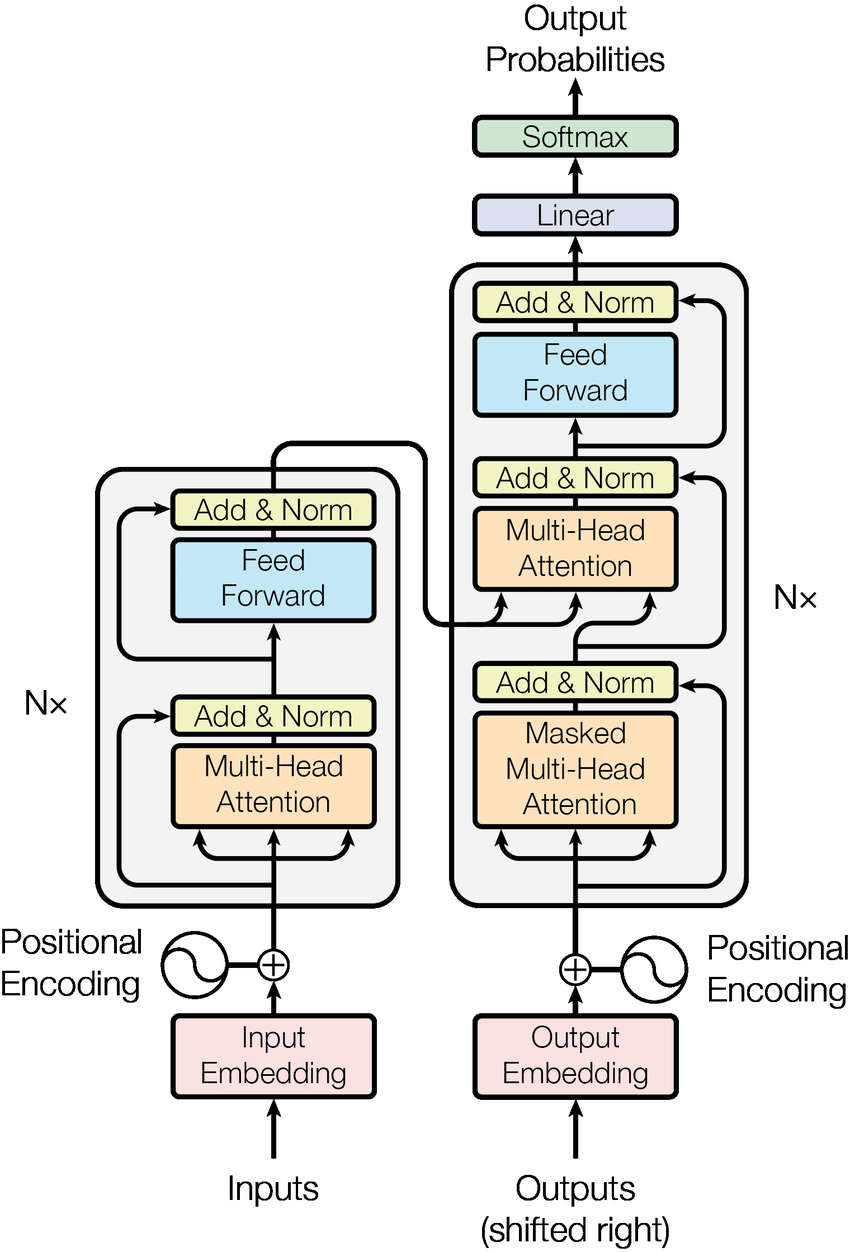
\includegraphics[height=0.5\textheight]{chapter-2/transformer.png}
    \caption{Arsitektur \textit{Transformers} \parencite{transformers}}
    \label{fig:transformer}
\end{figure}

Arsitektur dari \textit{Transformers} dapat dilihat pada Gambar \ref{fig:transformer}. Salah satu keunggulan utama dari mekanisme \textit{self-attention} adalah kemampuannya untuk menangani sekuens dengan panjang yang berbeda dan memahami hubungan antarkata tanpa mempertimbangkan jarak antara mereka. Ini memungkinkan \textit{Transformers} untuk memahami ketergantungan jarak jauh dalam teks, sesuatu yang sulit dicapai oleh arsitektur sebelumnya seperti RNN dan LSTM. Arsitektur dari \textit{Transformers} tersusun oleh \textit{encoder} dan \textit{decoder}, keduanya terdiri dari 6 tumpukan \textit{layer} yang identik. Setiap \textit{layer} pada \textit{encoder} mempunyai 2 \textit{sub-layer}, yaitu \textit{multi-head attention} dan \textit{feed forward}. Sedangkan, untuk \textit{decoder} mempunyai 3 \textit{sub-layer} dengan 2 \textit{sub-layer} yang sama pada \textit{encoder} dan 1 \textit{sub-layer} tambahan yang merupakan \textit{multi-head attention} terhadap keluaran dari \textit{encoder} \parencite{transformers}.

Mekanisme \textit{multi-head attention} terdiri dari beberapa \textit{attention head} yang dapat dideskripsikan sebagai pemetaan antara sebuah \textit{query} dan serangkaian \textit{key-value} ke sebuah keluaran. Perhitungan yang dilakukan untuk mendapatkan \textit{attention} adalah dengan menggunakan \textit{scaled dot-product attention} dengan rumus sebagai berikut \parencite{transformers}.

\begin{equation}
    Attention(Q, K, V) = softmax(\frac{QK^{T}}{\sqrt{d_k}})V
    \label{eq:attention}
\end{equation}

Pada rumus \ref{eq:attention}, Q, K, dan V masing-masing adalah matriks dari \textit{query, key}, dan \textit{value} yang diperoleh dari urutan masukan dan diproses secara linear ke dalam mekanisme \textit{self-attention} dari Transformers. Kemudian, bobot dari \textit{attention} dikalikan dengan matriks \textit{value} untuk mendapat jumlah bobot dari nilai-nilai tersebut. Dalam mekanisme \textit{multi-head attention}, proses perhitungan dilakukan secara paralel menggunakan beberapa \textit{attention head} yang menghasilkan bobot \textit{attention} yang berbeda. Kemudian, bobot tersebut akan digabungkan dan diproyeksikan kembali untuk menghasilkan keluaran akhir dari \textit{multi-head attention}.
